\documentclass[12pt,a4paper]{article}

\usepackage{fontspec}
\XeTeXlinebreaklocale "th"
\XeTeXlinebreakskip = 0pt plus 1pt
\defaultfontfeatures{Ligatures=TeX}
\setmainfont[
  Path={fonts/TH Sarabun PSK V-1/TH Sarabun PSK V-1/},
  Extension=.ttf,
  UprightFont={*},
  BoldFont={* Bold},
  ItalicFont={* Italic},
  BoldItalicFont={* BoldItalic}
]{THSarabun}
\setmonofont{Latin Modern Mono}

\usepackage{graphicx}
\usepackage{textcomp}
\usepackage{amsmath,amssymb,float,caption,subcaption,xcolor,hyperref,fancyhdr}
\usepackage{geometry,booktabs,array,tabularx}
\geometry{margin=1in}
\setlength{\headheight}{14.5pt}
\pagestyle{fancy}\fancyhf{}\lhead{การสลับโหมด GFL$\leftrightarrow$GFM อัตโนมัติด้วยดัชนี AGSI (IBR สองตัว)}\rhead{\thepage}
\hypersetup{colorlinks=true,linkcolor=blue,urlcolor=blue,citecolor=blue}
\renewcommand{\arraystretch}{1.12}
\captionsetup[table]{skip=7pt}
\emergencystretch=2em
\linespread{1.15}

\renewcommand{\abstractname}{บทคัดย่อ}
\renewcommand{\contentsname}{สารบัญ}
\renewcommand{\figurename}{รูปที่}
\renewcommand{\tablename}{ตารางที่}
\renewcommand{\refname}{เอกสารอ้างอิง}

\newcommand{\re}{\operatorname{Re}}
\newcommand{\im}{\operatorname{Im}}

\title{\textbf{การสลับโหมด Grid-Following $\leftrightarrow$ Grid-Forming อัตโนมัติของ IBR สองตัว
ด้วยดัชนีเสถียรภาพปรับตัว (AGSI) บน Infinite Bus}\\
\large หลักการ สมการทุกขั้นตอนโดยละเอียด และการถ่ายโอนแบบต่อเนื่องกระแส (bumpless)}
\date{23 กรกฎาคม 2569}

\begin{document}
\maketitle

\begin{abstract}
รายงานฉบับนี้ (แยกจากรายงานเปรียบเทียบ GFL/GFM แบบ 6 states ฉบับก่อนหน้า) อธิบาย \textbf{กลไกการสลับ
โหมดอัตโนมัติ} ระหว่าง Grid-Following (GFL) และ Grid-Forming (GFM) สำหรับ IBR สองตัวที่จุดเชื่อมต่อร่วม
(PCC) เดียวกัน ผ่านสายส่ง $Z_{line}$ สู่ ideal infinite bus \emph{โดยอธิบายทุกสมการและทุกขั้นตอนอย่าง
ละเอียด}: ตั้งแต่กรอบ DAE กระแสฉีดและกำลัง สมการโครงข่าย (KCL) การหาสมดุลเริ่มต้น สมการดัชนีเดียว
\textbf{Adaptive Grid Stability Index (AGSI)} พร้อมดัชนีย่อยและอัลกอริทึมคำนวณ เกณฑ์การสลับ (เส้นอ้างอิง
$\Gamma_{on},\Gamma_{off}$ ฮิสเทอรีซิส เวลาหน่วง) การพิสูจน์การถ่ายโอนแบบต่อเนื่องกระแส และตัวขับจำลอง
เชิงเวลา (implicit trapezoidal + Newton) ผลการจำลอง (project-owned MATLAB, ไม่มี external solver) ยืนยัน
วงจรสลับสองทางที่ลู่เข้าทุกสเต็ป กระแสต่อเนื่องระดับ $10^{-17}$ สมการทั้งหมดอ้างอิงได้และไม่มีการปรับค่า
เพื่อบิดผล
\end{abstract}
\newpage
\tableofcontents
\newpage

\section{ขอบเขตและความเชื่อมโยง}
รายงานก่อนหน้า (\texttt{report\_ibr\_gfl\_gfm\_th}) อธิบายลำดับ state และ SSSA ของแบบจำลอง IBR ลดรูป
\textbf{6 states} สองชุด (GFL และ GFM) ฉบับนี้ \emph{นำสองแบบจำลองนั้นมาใช้ซ้ำเป็นแกนสมการ} (single
source of truth) แล้วเพิ่ม \textbf{ชั้นควบคุมกำกับ (supervisor)} ที่สลับโหมดอัตโนมัติ จึงเน้น \emph{หลักการ
และสมการของการสลับ} โดยอธิบายทุกขั้นตอน

\textbf{Source discipline.} โครงสร้างการสลับ (AGSI, เส้นเกณฑ์, เวลาหน่วง) ยึด \emph{แนวทาง} งาน
EECON49-P4~\cite{eecon49th} ที่เสนอกลยุทธ์สลับ GFL/GFM ด้วย AGSI ร่วมกับ Bayesian Optimization (BO)
ฉบับนี้ใช้เป็น \emph{แนวทางเชิงออกแบบ ไม่ใช่ทำซ้ำเป๊ะ} (นำรูปสมการ AGSI และค่าเริ่มต้นจาก \S4.1 มาปรับใช้
กับระบบสองตัว โดย \emph{ไม่} ทำ BO) จึงจัดชั้น \texttt{PROJECT\_DERIVED\_SOURCE\_GUIDED}

\section{กรอบสมการและระบบทดสอบ}
\subsection{ทำไมต้องสลับโหมด}
GFL พึ่ง \emph{PLL} ซิงก์กับแรงดันกริด ทำงานดีเมื่อกริด \emph{แข็งแรง} แต่เมื่อกริด \emph{อ่อน}
(อิมพีแดนซ์สายสูง หรือสูญเสียแหล่งอ้างอิง) พลวัต PLL หน่วงน้อยลงและอาจไม่เสถียร ตรงข้ามกับ GFM (VSG) ที่
\emph{สร้างแรงดัน/ความถี่อ้างอิงได้เอง} จึงประคองกริดอ่อนได้ แนวคิดคือ ตรวจสภาวะแบบเรียลไทม์แล้วสลับ
GFL$\to$GFM เมื่อเครียด และ GFM$\to$GFL เมื่อกลับปกติ

\subsection{Disturbance ที่บังคับให้ GFL ต้องสลับ และกลไกทางฟิสิกส์}
\label{sec:disturb}
\textbf{Disturbance ที่ใช้ในรายงานนี้} คือ \emph{เหตุการณ์กริดอ่อนตัวชั่วคราว (temporary weak-grid event)}:
ที่เวลา $t_{ev}$ อิมพีแดนซ์สายส่งสู่ infinite bus ถูกคูณด้วยแฟกเตอร์ (default $\times4$: $Z_{line}$ จาก
$0.30j\to1.20j$ pu) จำลองการ \emph{สูญเสียเส้นทางส่งกำลังที่แข็งแรง} หรือการแยกส่วนกริดบางส่วน ทำให้เหลือ
กริดที่ \emph{อ่อน} (short-circuit ratio, SCR ต่ำลง เพราะ SCR $\propto 1/Z_{line}$ การคูณสาย $\times4$ ทำให้
SCR ลดเหลือ $\sim1/4$) นอกจากนี้กรอบงานยังรองรับ disturbance อื่น: การกระโดดเฟส/แรงดันของ $V_\infty$
(grid phase/voltage step) และการ \emph{สูญเสียแหล่งอ้างอิง} ($\mathrm{GRA}=0$ เช่น slack/SG ถูกปลด จน
กลายเป็นเกาะ) ในการสาธิตเลือก ``กริดอ่อนล้วน'' (ไม่มีเฟส snap) เพื่อให้ transient เบาและกราฟอ่านง่าย

\textbf{ทำไม disturbance นี้จึงบังคับให้ GFL ต้องสลับ (ลำดับเหตุผล):}
\begin{enumerate}
\item GFL ทำตัวเป็น \emph{แหล่งกระแส} ที่ควบคุมกำลัง $P,Q$ ให้คงที่ เมื่อสาย \emph{อ่อน} (อิมพีแดนซ์สูง)
การส่งกำลังเท่าเดิมผ่านสายอิมพีแดนซ์สูงทำให้ \emph{แรงดันตกคร่อมสายมาก} $\Rightarrow$ แรงดัน PCC ตก
(ในการจำลอง $\lvert V\rvert$ ตกจาก $\sim0.99$ เหลือ $\sim0.79$ pu)
\item แรงดันตกทำให้ \emph{ดัชนีย่อยแรงดัน} พุ่งขึ้นทันที (พจน์เด่นสุด):
$J_V=\lvert V-1\rvert/0.10$ จาก $\sim0.02$ ขึ้นเป็น $\sim2.1$
\item เมื่อกริดอ่อนลง จุดทำงานเข้าใกล้ \emph{ขีดจำกัดกำลังสูงสุด (max-power / voltage-collapse nose)} และ
พลวัต PLL ของ GFL \emph{หน่วงน้อยลง} ทำให้เกิด transient ความถี่และ RoCoF $\Rightarrow$ $J_f, J_R$ สูงขึ้น
ด้วย (นี่คือปรากฏการณ์ weak-grid GFL instability ที่ทราบกันดี~\cite{liu2024b})
\item ผลรวมถ่วงน้ำหนัก AGSI จึงไต่ขึ้น \emph{ชนเส้น} $\Gamma_{on}$ $\Rightarrow$ สั่งสลับเป็น \textbf{GFM}
\end{enumerate}

\textbf{ทำไม GFM ช่วยได้:} GFM เป็น \emph{แหล่งแรงดัน} (voltage source behind impedance) ที่สร้างแรงดัน/
ความถี่อ้างอิงเองพร้อม virtual inertia จึงทำงานบนกริดอ่อนได้ หยุดการทรุดของแรงดัน และคืนเสถียรภาพ เมื่อสาย
กลับสู่ปกติ (recovery) กริดกลับแข็งแรง GFL ก็ทำงานได้ดีอีกครั้ง AGSI ตกใต้ $\Gamma_{off}$ จึงสลับกลับ GFL

\subsection{กรอบ DAE ร่วม กระแสฉีด และกำลัง}
\label{sec:dae}
แต่ละ IBR ใช้ระบบสมการเชิงอนุพันธ์-พีชคณิต (DAE) แบบ input-driven ร่วมกัน
\begin{equation}
\dot{x} = f(x,y,u), \qquad 0 = g(x,y,u),
\label{eq:dae}
\end{equation}
โดย $x$ คือ \emph{สถานะพลวัต} ของอุปกรณ์ (6 ตัว), $y=[\re(V)\ \im(V)]^T$ คือ \emph{สถานะพีชคณิต} (แรงดัน
บัส) และ $u=[P_{ref}\ Q_{ref}]^T$ คือ \emph{อินพุตอ้างอิง} สมการ~\eqref{eq:dae} หมายความว่า: แถวบน
($\dot x=f$) กำหนดว่าสถานะเปลี่ยนแปลงอย่างไรตามเวลา ส่วนแถวล่าง ($0=g$) คือข้อจำกัดพีชคณิต (KCL ของ
โครงข่าย) ที่ต้องเป็นจริงทุกขณะ

\textbf{ขั้นตอนแปลงกรอบ dq $\leftrightarrow$ เฟสเซอร์.} กำหนดมุมอ้างอิงของอุปกรณ์ $\delta$ (GFL ใช้มุม
PLL, GFM ใช้มุมโรเตอร์) แล้วฉายแรงดันเข้ากรอบ dq ทีละขั้น
\begin{equation}
V_{dq} = V\,e^{-j\delta},\qquad v_d = \re(V_{dq}),\quad v_q = \im(V_{dq}),
\label{eq:vdq}
\end{equation}
กระแสฉีดสู่โครงข่าย (คืนค่าบน system base) แปลงกลับด้วย
\begin{equation}
I \;=\; \frac{(i_d + j\,i_q)\,e^{j\delta}}{\kappa},\qquad \kappa=\frac{S_{base}}{M_{base}},
\label{eq:iinj}
\end{equation}
โดย $i_d,i_q$ คือกระแสในกรอบ dq (บน inverter base) และ $\kappa$ คือตัวคูณเปลี่ยนฐาน (system/inverter)
กำลังเชิงซ้อนที่ปลายทางคำนวณจากนิยามกำลังเฟสเซอร์ (generator convention)
\begin{equation}
S = V\,\overline{I},\qquad P=\re(S),\quad Q=\im(S),
\label{eq:power}
\end{equation}
โดย $\overline{(\cdot)}$ คือสังยุค (complex conjugate) สมการ~\eqref{eq:iinj}--\eqref{eq:power} จะถูกใช้ซ้ำ
ในการพิสูจน์ความต่อเนื่องกระแส (\S\ref{sec:bumpless})

\subsection{ระบบทดสอบ: IBR สองตัวที่ PCC ร่วม + infinite bus}
\label{sec:kcl}
IBR สองตัว (\texttt{IBR1}, \texttt{IBR2}) เริ่มเป็น GFL ทั้งคู่ อยู่บัสเดียวกัน (PCC แรงดัน $V$) แล้วผ่าน
สายส่ง $Z_{line}$ สู่ infinite bus $V_\infty$ (แรงดันคงที่)

\textbf{ที่มาของสมการโครงข่าย (KCL) ทีละขั้น.} ตามกฎกระแสของ Kirchhoff ที่โหนด PCC: ผลรวมกระแสที่
\emph{ฉีดเข้า} โหนด ต้องเท่ากับกระแสที่ \emph{ไหลออก} ทางสายส่ง กระแสในสายส่งหาได้จากกฎของ Ohm
$I_{line} = (V - V_\infty)/Z_{line}$ ดังนั้น
\begin{equation}
\underbrace{I_1(x_1,V) + I_2(x_2,V)}_{\text{กระแสฉีดรวมจาก IBR}}
\;=\;
\underbrace{\frac{V - V_\infty}{Z_{line}}}_{\text{กระแสไหลออกทางสาย}}
\label{eq:kcl}
\end{equation}
สมการ~\eqref{eq:kcl} คือ $g(x,y,u)=0$ ในกรอบ~\eqref{eq:dae} สำหรับระบบนี้ (มีโหนดพีชคณิตเดียวคือ $V$)
เขียนแยกส่วนจริง/จินตภาพได้สองสมการจริง

\subsection{การหาสมดุลเริ่มต้นที่ PCC (ก่อนเหตุการณ์)}
\label{sec:equil}
ก่อนเกิดเหตุการณ์ ระบบต้องอยู่ที่ \emph{จุดสมดุล} (แบน ไม่มี transient) เราหาแรงดัน PCC เริ่มต้น $V$ จาก
สมดุลกำลัง โดยอนุมานทีละขั้น:
\begin{align}
\text{กระแสสาย:}\quad & I_{line} = \frac{V - V_\infty}{Z_{line}}, \label{eq:iline}\\
\text{กำลังไหลออกสู่สาย:}\quad & S_{line} = V\,\overline{I_{line}}, \label{eq:sline}\\
\text{สมดุลที่ PCC (ฉีด = ไหลออก):}\quad & S_1 + S_2 = S_{line} = V\,\overline{I_{line}}. \label{eq:sbal}
\end{align}
แทน~\eqref{eq:iline} ใน~\eqref{eq:sbal} แล้วนำสังยุคทั้งสองข้าง ได้สมการเดียวสำหรับ $V$
\begin{equation}
\boxed{\;\overline{V}\,\frac{(V - V_\infty)}{Z_{line}} \;=\; \overline{S_1 + S_2}\;}
\label{eq:pcceq}
\end{equation}
สมการ~\eqref{eq:pcceq} \emph{ไม่เป็นเชิงเส้น} และมีสังยุคของ $V$ จึงแก้ด้วย \textbf{Newton บนตัวแปรจริงสอง
ตัว} $\,\mathbf{v}=[\re(V);\ \im(V)]$: กำหนด residual $\,\mathbf{r}(\mathbf{v})=[\re(F);\ \im(F)]$ โดย
$F(V)=\overline{V}(V-V_\infty)/Z_{line}-\overline{S_{tot}}$ แล้ววนซ้ำ
$\mathbf{v}\leftarrow\mathbf{v}-J^{-1}\mathbf{r}$ (Jacobian $J$ จากผลต่างจำกัดกึ่งกลาง) จนกว่า
$\lVert\mathbf{r}\rVert_\infty$ เล็กกว่า tolerance เมื่อได้ $V$ แล้ว จึงตั้งสถานะเริ่มต้นของแต่ละ IBR จาก
$\texttt{equilibrium\_initialize}(V,P_k,Q_k)$ และตรวจว่า residual ของ~\eqref{eq:kcl} และ $f$ อยู่ระดับ
machine precision (ผลจริง: $\lvert$KCL$\rvert\sim10^{-15}$)

\subsection{คลาสอุปกรณ์สลับได้ (\texttt{SwitchableIbr6})}
อุปกรณ์แต่ละตัวห่อหุ้มแบบจำลองทั้งสองโหมด สถานะแอ็กทีฟ \emph{มี 6 ตัวเสมอ} การสลับไม่เปลี่ยนขนาดเวกเตอร์
แต่ \emph{re-initialise} 6 ช่องให้เป็นสมดุลของโหมดปลายทาง (\S\ref{sec:bumpless}) หน้าที่: (ก) ส่งต่อ
$f,\ I$ ไปโหมดแอ็กทีฟ (ข) ประเมิน AGSI (ค) ถ่ายโอนโหมด

\section{สมการการสลับ: ดัชนี AGSI และเส้นอ้างอิง}
\label{sec:agsi}
\subsection{นิยามดัชนี AGSI}
Adaptive Grid Stability Index รวมความเบี่ยงเบนที่วัดได้ ณ PCC สี่ปริมาณ ให้เป็นดัชนีไร้หน่วยเดียว
\begin{equation}
\boxed{\;\mathrm{AGSI} \;=\; w_V J_V \;+\; w_f J_f \;+\; w_R J_R \;+\; w_P J_P\;}
\label{eq:agsi}
\end{equation}
ดัชนีย่อยแต่ละตัว \emph{ทำ normalisation} ด้วยค่าฐานเฉพาะ (characteristic deviation)
\begin{align}
J_V &= \frac{\lvert V - V_{ref}\rvert}{\Delta V_{base}}
   &&\text{(ความเบี่ยงเบนแรงดัน)}\label{eq:jv}\\
J_f &= \frac{\lvert f - f_0\rvert}{\Delta f_{base}}
   &&\text{(ความเบี่ยงเบนความถี่)}\label{eq:jf}\\
J_R &= \frac{\lvert \mathrm{d}f/\mathrm{d}t\rvert}{\Delta \mathrm{RoCoF}_{base}}
   &&\text{(อัตราการเปลี่ยนความถี่, RoCoF)}\label{eq:jr}\\
J_P &= \frac{\lvert P_{ref} - P\rvert}{\Delta P_{base}}
   &&\text{(ความคลาดเคลื่อนกำลังจริง)}\label{eq:jp}
\end{align}
และน้ำหนักรวมเป็นหนึ่ง $w_V + w_f + w_R + w_P = 1$ ค่าที่ใช้เป็น default (แนวทางจาก \S4.1
ของ~\cite{eecon49th}) สรุปในตารางที่~\ref{tab:agsi}

\begin{table}[H]\centering
\caption{พารามิเตอร์ของสมการ AGSI และเกณฑ์การสลับ (default)}
\label{tab:agsi}
\begin{tabular}{@{}lll@{}}
\toprule
กลุ่ม & สัญลักษณ์ & ค่า default \\
\midrule
น้ำหนัก & $w_V,\ w_f,\ w_R,\ w_P$ & $0.30,\ 0.30,\ 0.25,\ 0.15$ \\
ค่าฐาน normalisation & $\Delta V_{base}$ & $0.10$ pu \\
 & $\Delta f_{base}$ & $0.50$ Hz \\
 & $\Delta \mathrm{RoCoF}_{base}$ & $1.00$ Hz/s \\
 & $\Delta P_{base}$ & $0.20$ pu \\
อ้างอิง & $V_{ref},\ f_0$ & $1.0$ pu, $60$ Hz \\
เส้นเกณฑ์ & $\Gamma_{on}$ (ขึ้น GFM) & $0.65$ \\
 & $\Gamma_{off}$ (ลง GFL) & $0.35$ \\
เวลาหน่วง & $T_{d,on},\ T_{d,off}$ & $0.10$ s, $1.00$ s \\
\bottomrule
\end{tabular}
\end{table}

\subsection{ความหมายของแต่ละพจน์}
\label{sec:meaning}
สมการ~\eqref{eq:agsi} รวม \emph{ความเบี่ยงเบนของสภาวะกริดสี่ด้าน} ที่วัดได้ ณ PCC โดยแต่ละพจน์บอก
``มุมมองความเครียด'' คนละแบบ

\begin{itemize}
\item \textbf{AGSI} --- ดัชนีเสถียรภาพรวม (ไร้หน่วย) ยิ่งสูงยิ่งเครียด/เข้าใกล้ไม่เสถียร ใช้เป็นตัวเดียว
ในการตัดสินสลับโหมด

\item \textbf{$J_V=\lvert V-V_{ref}\rvert/\Delta V_{base}$ --- ดัชนีย่อยแรงดัน.} $V$ คือขนาดแรงดันที่ PCC
เทียบค่าปกติ $V_{ref}=1.0$ pu กริดอ่อน/โหลดหนักทำแรงดันตก $\Rightarrow J_V$ สูง (ในระบบเรานี่คือ
\emph{ตัวขับหลัก}) ค่าฐาน $\Delta V_{base}=0.10$ pu (เพี้ยน $10\%\Rightarrow J_V=1$)

\item \textbf{$J_f=\lvert f-f_0\rvert/\Delta f_{base}$ --- ดัชนีย่อยความถี่.} $f$ ในโหมด GFL มาจาก PLL,
ในโหมด GFM มาจากความถี่โรเตอร์เสมือน VSG เทียบพิกัด $f_0=60$ Hz บ่งชี้ \emph{ความไม่สมดุลกำลัง}/แนวโน้ม
หลุด synchronism ค่าฐาน $\Delta f_{base}=0.50$ Hz

\item \textbf{$J_R=\lvert \mathrm{d}f/\mathrm{d}t\rvert/\Delta \mathrm{RoCoF}_{base}$ --- ดัชนีย่อย RoCoF.}
อัตราการเปลี่ยนความถี่ เป็นดัชนีมาตรฐานของความเฉื่อยระบบ ระบบ IBR สูง (inertia ต่ำ) มี RoCoF \emph{ใหญ่}
หลังการรบกวน อันตรายต่อเสถียรภาพความถี่~\cite{entsoe_rocof} $\Rightarrow$ ควรสลับเป็น GFM ที่ให้ virtual
inertia ค่าฐาน $\Delta \mathrm{RoCoF}_{base}=1.0$ Hz/s (ระดับเกณฑ์ทนทาน RoCoF ของ grid code $\sim0.5$--$2$ Hz/s)

\item \textbf{$J_P=\lvert P_{ref}-P\rvert/\Delta P_{base}$ --- ดัชนีย่อยความคลาดกำลัง.} เทียบกำลังที่ \emph{สั่ง}
กับที่ \emph{ฉีดจริง} คลาดมากบ่งชี้ตัวแปลง \emph{ส่งกำลังตามคำสั่งไม่ไหว} ค่าฐาน $\Delta P_{base}=0.20$ pu

\item \textbf{$w_V,w_f,w_R,w_P$ (รวม $=1$).} น้ำหนักความสำคัญแต่ละด้าน default $0.30/0.30/0.25/0.15$ (เน้น
แรงดัน+ความถี่มากสุด) ในต้นฉบับปรับด้วย BO ที่นี่ตรึงเป็นแนวทาง

\item \textbf{ค่าฐาน normalisation.} ทำให้ดัชนีย่อยไร้หน่วยและเทียบกันได้: เบี่ยงเบนเท่าค่าฐาน $\Rightarrow$
ดัชนีย่อย $=1$ (เหมือน ``เพี้ยนกี่เท่าของค่าที่ยอมรับ'')

\item \textbf{$\Gamma_{on}=0.65,\ \Gamma_{off}=0.35$ --- เส้นอ้างอิง.} เกณฑ์บน/ล่างของ AGSI

\item \textbf{$\mathrm{GRA}\in\{0,1\}$.} ความพร้อมแหล่งอ้างอิงกริด ($1=$ มี infinite bus/GFM; $0=$ สูญเสีย/
แยกเกาะ $\Rightarrow$ บังคับ GFM)

\item \textbf{$T_{d,on}=0.10$ s, $T_{d,off}=1.0$ s.} เวลาหน่วงที่เงื่อนไขต้องคงอยู่ต่อเนื่องก่อนสลับ
\end{itemize}

\subsection{อัลกอริทึมการคำนวณ AGSI (ทีละขั้น)}
\label{sec:algo}
ทุกสเต็ปเวลา $t_n$ คำนวณ AGSI ดังนี้:
\begin{enumerate}
\item อ่านสถานะโหมดปัจจุบัน แล้ว reconstruct: แรงดัน $V$ (จาก $y$), ความถี่ $f$, กำลังจริง $P=\re(V\overline{I})$
\item $J_V=\lvert V\rvert$ ต่างจาก $V_{ref}$ หารด้วย $\Delta V_{base}$ ตาม~\eqref{eq:jv}
\item $J_f$ ตาม~\eqref{eq:jf}
\item \textbf{RoCoF เชิงตัวเลข:} $\dfrac{\mathrm{d}f}{\mathrm{d}t}\approx\dfrac{f(t_n)-f(t_{n-1})}{t_n-t_{n-1}}$
โดยใช้ความถี่ของ \emph{สเต็ปก่อนหน้า} ($f_{prev}$) ที่บันทึกไว้ (อัปเดตครั้งเดียวต่อสเต็ปเพื่อไม่ให้ค่า
ผิดเพี้ยนจากการเรียกซ้ำ) แล้วได้ $J_R$ ตาม~\eqref{eq:jr}
\item $J_P$ จาก $P_{ref}=u(1)$ เทียบ $P$ ตาม~\eqref{eq:jp}
\item รวมถ่วงน้ำหนักตาม~\eqref{eq:agsi}
\end{enumerate}

\subsection{เกณฑ์การสลับ (index ทำงานอย่างไร)}
กำหนด $\mathrm{GRA}\in\{0,1\}$ การตัดสินใจ (ทีละขั้น):
\begin{enumerate}
\item \textbf{ประเมิน} $\mathrm{AGSI}$ ตาม \S\ref{sec:algo} ทุกสเต็ป
\item \textbf{เงื่อนไขสลับขึ้น (GFL$\to$GFM):}
\begin{equation}
\big(\mathrm{AGSI}\ge\Gamma_{on}\big)\ \lor\ \big(\mathrm{GRA}=0\big)
\quad\text{คงอยู่ต่อเนื่อง}\ \ge T_{d,on}
\label{eq:up}
\end{equation}
คือดัชนี \emph{ชนเส้นบน} $\Gamma_{on}$ (เครียด) \emph{หรือ} สูญเสียแหล่งอ้างอิง และคงอยู่ครบ $T_{d,on}$
\item \textbf{เงื่อนไขสลับลง (GFM$\to$GFL):}
\begin{equation}
\big(\mathrm{AGSI}<\Gamma_{off}\big)\ \land\ \big(\mathrm{GRA}=1\big)
\quad\text{คงอยู่ต่อเนื่อง}\ \ge T_{d,off}
\label{eq:down}
\end{equation}
คือดัชนี \emph{ตกใต้เส้นล่าง} $\Gamma_{off}$ (สงบ) \emph{และ} มีแหล่งอ้างอิง และคงอยู่ครบ $T_{d,off}$
\end{enumerate}

\textbf{หมายเหตุ (โหมด default = ขับด้วยดัชนีล้วน, per-IBR).} โดย default การสลับ \emph{ขับด้วย AGSI เทียบ
เส้นเกณฑ์เท่านั้น} (ปิดเงื่อน GRA): เมื่อสูญเสียแหล่งอ้างอิง เช่น SG หลุดในระบบหลายเครื่อง \emph{ไม่ได้บังคับ
ให้ IBR ทุกตัวเป็น GFM} แต่เฉพาะ IBR ที่เครียดจน AGSI \emph{แตะเส้น} $\Gamma_{on}$ เท่านั้นที่สลับ ดัชนีจึง
\emph{เลือกชุด GFM ขั้นต่ำที่จำเป็น} ให้เองตามสภาพจริงของแต่ละตัว ส่วนเงื่อน GRA แบบบังคับใน
สมการ~\eqref{eq:up}--\eqref{eq:down} เป็น \emph{ตัวเลือกเสริม} (\texttt{gra\_override}, ปิดไว้เป็นค่าเริ่มต้น)
ตามรูปแบบดั้งเดิมของ EECON49 นอกจากนี้ในการศึกษานี้ตั้ง \emph{ไม่มีเวลาหน่วง} ($T_{d,on}=T_{d,off}=0$) เพื่อ
ดูการสลับแบบทันที (ดู \S\ref{sec:agsipp}: AGSI++ ทำให้การสลับทันทีไม่สั่น โดยไม่ต้องพึ่ง dwell)


\textbf{กลไกเวลาหน่วง (dwell) ทีละขั้น.} เก็บเวลา $t_{since}$ ที่เงื่อนไขเริ่มเป็นจริง: ถ้าเงื่อนไขเป็นจริง
และ $t_{since}$ ยังไม่ถูกตั้ง ให้ตั้ง $t_{since}=t$; ถ้าเงื่อนไขเป็นเท็จ ให้รีเซ็ต $t_{since}=$ ว่าง;
จะสลับก็ต่อเมื่อ $t-t_{since}\ge T_{d}$ (และเวลาที่อยู่ในโหมดปัจจุบัน $\ge T_d$) กลไกนี้ทำให้ \emph{spike
ชั่วขณะ} (เช่น RoCoF พุ่งตอนกริดคืน) ไม่ทำให้สลับ เพราะไม่ ``คงอยู่'' ครบเวลา

\textbf{ฮิสเทอรีซิส.} เนื่องจาก $\Gamma_{on}>\Gamma_{off}$ เกิด \emph{แถบ} $[\Gamma_{off},\Gamma_{on}]$
ที่ \emph{ไม่มีการสลับ} เมื่อ AGSI อยู่ในแถบ ป้องกันการสลับไปมาถี่ ๆ ดูรูปที่~\ref{fig:agsi}

\begin{figure}[H]\centering
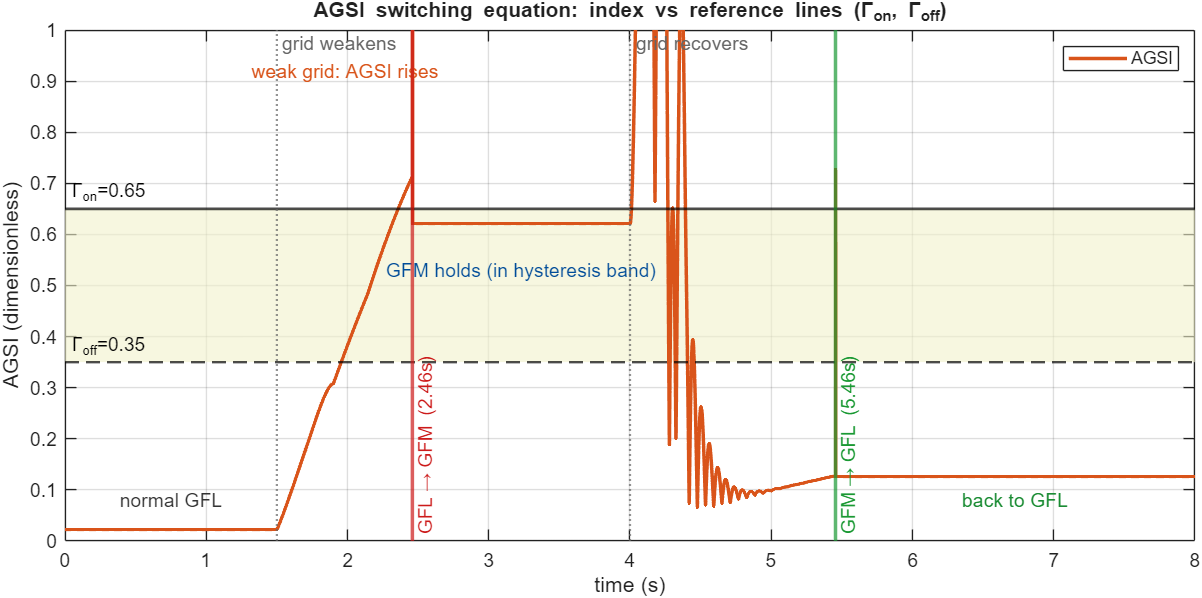
\includegraphics[width=\textwidth]{figures/two_ibr_switch/agsi_annotated.png}
\caption{สมการดัชนี AGSI เทียบเส้นอ้างอิง $\Gamma_{on}=0.65$ (ทึบ) และ $\Gamma_{off}=0.35$ (ประ) แถบ
เหลืองคือช่วงฮิสเทอรีซิส ดัชนีไต่ขึ้นชน $\Gamma_{on}$ แล้วสลับเป็น GFM (เส้นแดง) ค้างในแถบระหว่างกริดอ่อน
จากนั้นเมื่อกริดคืน ตกใต้ $\Gamma_{off}$ แล้วสลับกลับ GFL (เส้นเขียว)}
\label{fig:agsi}
\end{figure}

\subsection{AGSI++ : ส่วนขยายที่นำมาใช้เป็นหลัก}
\label{sec:agsipp}
AGSI เดิม (\S\ref{sec:agsi}) เป็นรูปสมการของ EECON49-P4 พอดี ในรายงานนี้ปรับปรุงเป็น \textbf{AGSI++}
โดยเพิ่มสามส่วนที่ทำให้ ``ดีกว่าเดิม'' สำหรับการสลับบนกริดอ่อนจริง
\begin{equation}
\mathrm{AGSI}^{++} = w_V J_V + w_f J_f + w_R J_R^{\text{filt}} + w_P J_P
   + w_{SCR}\,J_{SCR} + w_{lock}\,J_{lock}
\label{eq:agsipp}
\end{equation}
โดยน้ำหนัก (รวม $=1$) default คือ $[w_V,w_f,w_R,w_P,w_{SCR},w_{lock}]=[0.25,0.25,0.15,0.10,0.15,0.10]$
สามส่วนที่เพิ่ม:
\begin{enumerate}
\item \textbf{Filtered RoCoF ($J_R^{\text{filt}}$).} แทน RoCoF ดิบด้วยค่าผ่าน low-pass อันดับหนึ่ง
\begin{equation}
\mathrm{RoCoF}^{\text{filt}}_{n}=\mathrm{RoCoF}^{\text{filt}}_{n-1}
  +\alpha\big(\mathrm{RoCoF}^{\text{raw}}_{n}-\mathrm{RoCoF}^{\text{filt}}_{n-1}\big),
\quad \alpha=\min\!\Big(1,\tfrac{\Delta t}{\tau_R}\Big),\ \tau_R=0.05\text{ s}
\label{eq:rocoffilt}
\end{equation}
กำจัด spike หนึ่ง-แซมเปิลตอนเปลี่ยนโครงสร้าง (ต้นเหตุของ chattering เมื่อไม่มี dwell)
\item \textbf{ดัชนีความแข็งแรงกริด ($J_{SCR}$).} วัด \emph{ต้นเหตุ} (กริดอ่อน) โดยตรง
\begin{equation}
J_{SCR}=\max\!\Big(0,\ \tfrac{\mathrm{SCR}_{crit}}{\mathrm{SCR}}-1\Big),\qquad
\mathrm{SCR}=\frac{|V_\infty|^2}{|Z_{line}|\,S_{agg}},\ \ \mathrm{SCR}_{crit}=3
\label{eq:jscr}
\end{equation}
เมื่อ SCR ตกใต้เกณฑ์อ่อน $J_{SCR}$ เป็นบวก (งานนี้คำนวณ SCR จากโครงข่ายที่ทราบ = diagnostic; ระบบจริง
ประมาณจาก $\mathrm{d}V/\mathrm{d}I$)
\item \textbf{ดัชนีหลุด-ล็อกของ PLL ($J_{lock}=|v_q|/\Delta v_{q,base}$).} แรงดันแกน q ในเฟรม PLL (ปกติ
$\approx0$) เป็นตัวชี้ ``หลุด lock'' โดยตรงของ GFL
\end{enumerate}

\textbf{ผลเทียบบนระบบ 2-IBR (เหตุการณ์เดียวกัน).} ตารางที่~\ref{tab:agsipp} และรูปที่~\ref{fig:agsipp}:
\textbf{AGSI++ สลับสะอาด (2 ครั้ง/ตัว) โดยไม่ต้องมี dwell} ส่วน AGSI เดิมแบบไม่มี dwell \emph{สั่น (chatter,
4 ครั้ง)} เพราะ RoCoF spike (AGSI พุ่งถึง $\sim38$) การกรอง RoCoF ทำให้ AGSI++ สูงสุดเพียง $\sim1.5$ จึงนำ
AGSI++ มาเป็น \emph{ดัชนีหลัก}

\begin{table}[H]\centering
\caption{เทียบ AGSI เดิม กับ AGSI++ บนระบบ 2-IBR (กริดอ่อน $\times4$, ramp 0.4 s)}
\label{tab:agsipp}
\begin{tabular}{@{}lccl@{}}
\toprule
กรณี & ครั้งสลับ/ตัว & max AGSI & สรุป \\
\midrule
AGSI เดิม, ไม่มี dwell & 4 & 37.75 & สั่น (chatter) จาก RoCoF spike \\
AGSI เดิม, มี dwell    & 2 & 24.97 & สะอาด แต่ต้องพึ่ง dwell + ช้ากว่า \\
\textbf{AGSI++, ไม่มี dwell} & \textbf{2} & \textbf{1.45} & \textbf{สะอาดโดยไม่ต้อง dwell} \\
AGSI++, มี dwell       & 2 & 1.55 & สะอาด \\
\bottomrule
\end{tabular}
\end{table}

\begin{figure}[H]\centering
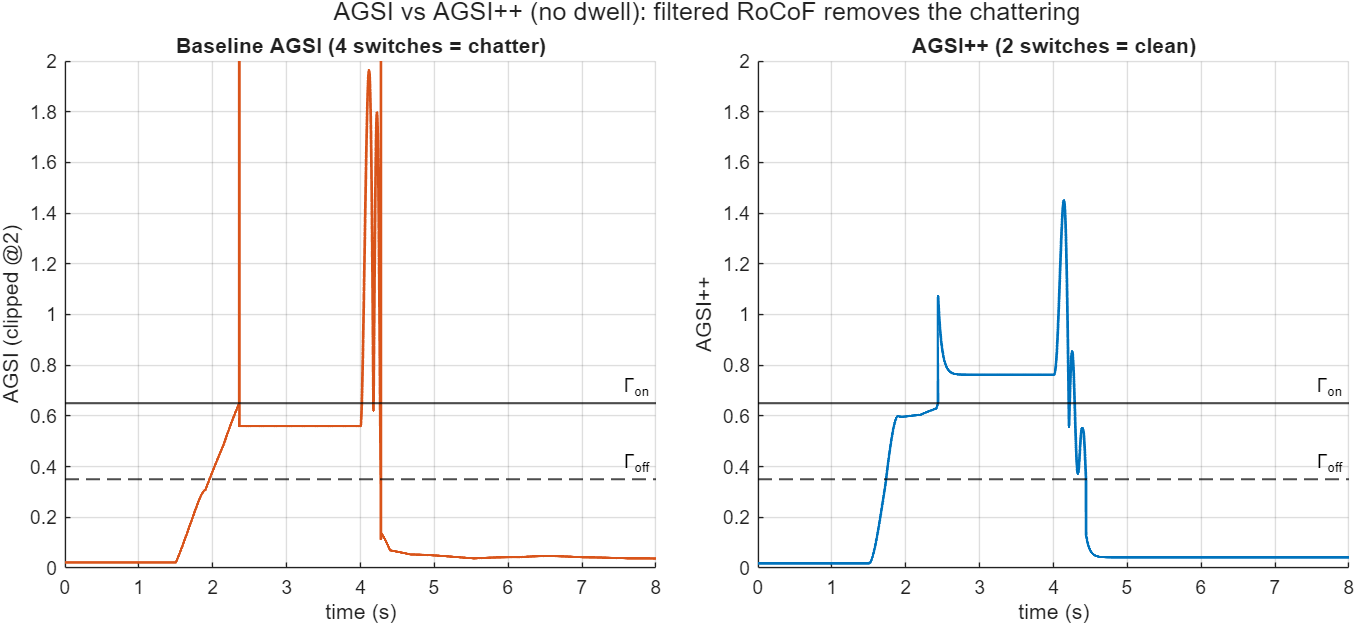
\includegraphics[width=\textwidth]{figures/two_ibr_switch/agsi_pp_compare.png}
\caption{เทียบดัชนีแบบไม่มี dwell: (ซ้าย) AGSI เดิม พุ่งเกินสเกล (clip ที่ 2) สลับ 4 ครั้ง (chatter);
(ขวา) AGSI++ (filtered RoCoF) มีขอบเขต ($<1.5$) สลับสะอาด 2 ครั้ง}
\label{fig:agsipp}
\end{figure}


\section{การถ่ายโอนแบบต่อเนื่องกระแส (bumpless transfer)}
\label{sec:bumpless}
ขณะสลับที่เวลา $t^\star$ ทำทีละขั้น:
\begin{enumerate}
\item อ่านแรงดันปลายทาง $V$ (จาก $y$) และกระแสฉีดปัจจุบันของโหมดเดิม
$I^- = I_{\text{เดิม}}(x^-,V)$
\item คำนวณกำลัง ณ ขณะนั้น $S = V\,\overline{I^-}$, $P=\re(S)$, $Q=\im(S)$
\item ตั้งสถานะโหมดปลายทางให้เป็น \emph{สมดุล} ที่ส่งมอบ $(P,Q)$ เดิม ที่แรงดัน $V$ เดิม ผ่าน
\texttt{equilibrium\_initialize}$(V,P,Q)$
\end{enumerate}

\textbf{พิสูจน์ความต่อเนื่องกระแส (ทุกขั้น).} พิจารณาโหมด GFL: สมดุลกำหนด
$i_{d0}=\kappa P/\lvert V\rvert$, $i_{q0}=-\kappa Q/\lvert V\rvert$, และมุม $\delta=\angle V$ แทนใน~\eqref{eq:iinj}
\begin{align}
I^+ &= \frac{(i_{d0}+j\,i_{q0})\,e^{j\delta}}{\kappa}
     = \frac{\big(\tfrac{\kappa P}{\lvert V\rvert}-j\tfrac{\kappa Q}{\lvert V\rvert}\big)e^{j\angle V}}{\kappa}
     = \frac{(P-jQ)}{\lvert V\rvert}\,e^{j\angle V} \notag\\
    &= (P-jQ)\,\frac{V}{\lvert V\rvert^2}
     = \frac{P-jQ}{\overline{V}}
     = \overline{\left(\frac{P+jQ}{V}\right)}
     = \overline{\left(\frac{S}{V}\right)} = I^-.
\label{eq:cont}
\end{align}
โดยใช้ $e^{j\angle V}=V/\lvert V\rvert$ และ $V/\lvert V\rvert^2=1/\overline{V}$ โหมด GFM ก็ให้ผลเดียวกัน
(สมดุลตั้งจาก $I_{net}=\overline{(P+jQ)/V}$ โดยตรง) ดังนั้น \emph{กระแสฉีดต่อเนื่องข้ามการสลับทั้งสองทิศ}
(ไม่มีการกระโดดของกระแสในโครงข่าย) ผลทดสอบ: $\lvert I^+ - I^-\rvert\approx2.8\times10^{-17}$

\textbf{การ back-solve ค่าอ้างอิง GFM (ให้อนุพันธ์เป็นศูนย์ที่ขณะสลับ).} สมการแรงดัน GFM มี
$\tau_E\dot E = k_Q(Q_{ref}-Q) - k_E(E-\lvert V\rvert)$ ต้องการ $\dot E=0$ ที่ขณะสลับ (โดย $E_0$ คือค่าเริ่มต้น
ที่ตั้งไว้) จึงแก้หา
\begin{equation}
k_Q(Q_{ref}-Q) = k_E(E_0-\lvert V\rvert)
\;\Rightarrow\;
Q_{ref} = Q + \frac{k_E\,(E_0-\lvert V\rvert)}{k_Q\,\kappa},
\label{eq:qref}
\end{equation}
และตั้ง $P_{ref}=P$ เพื่อให้สมการ swing ($M\dot\omega = P_{ref}-P-D_v(\omega-1)$) มี $\dot\omega=0$ ที่
$\omega=1$ ดังนั้น GFM เริ่มที่สมดุลพอดี (bumpless เต็มรูป)

\section{ตัวขับจำลองเชิงเวลา (TDS driver)}
\label{sec:driver}
\subsection{Implicit-trapezoidal คู่กับ KCL}
รวมสถานะเป็น $z=[x_1;\,x_2;\,y]$ (มิติ $6+6+2=14$) การก้าวจาก $t_n$ ไป $t_{n+1}=t_n+\Delta t$ ใช้กฎ
สี่เหลี่ยมคางหมูโดยปริยาย (implicit trapezoidal) สำหรับสถานะพลวัต คู่กับ KCL~\eqref{eq:kcl} เป็น residual
\begin{equation}
\mathbf{r}(z_{n+1}) =
\begin{bmatrix}
x_{1,n+1} - x_{1,n} - \tfrac{\Delta t}{2}\big(f_1(x_{1,n})+f_1(x_{1,n+1})\big)\\[2pt]
x_{2,n+1} - x_{2,n} - \tfrac{\Delta t}{2}\big(f_2(x_{2,n})+f_2(x_{2,n+1})\big)\\[2pt]
g(x_{1,n+1},x_{2,n+1},V_{n+1})
\end{bmatrix} = \mathbf{0}.
\label{eq:trap}
\end{equation}
แถวสองบนคือสูตรคางหมู $x_{n+1}=x_n+\tfrac{\Delta t}{2}(f_n+f_{n+1})$ (อันดับสอง, A-stable) แถวล่างบังคับ
KCL ที่ปลายสเต็ป แก้~\eqref{eq:trap} ด้วย \textbf{damped Newton}: วนซ้ำ $z\leftarrow z+\alpha\,\Delta z$
โดย $\Delta z=-J^{-1}\mathbf{r}$, $J=\partial \mathbf{r}/\partial z$ ประมาณด้วยผลต่างจำกัด, และ $\alpha$ ลด
ครึ่งถ้าค่าไม่จำกัด จนกว่า $\lVert\mathbf{r}\rVert_\infty\le$ tolerance ผลจริง: ลู่เข้าทุกสเต็ป

\subsection{เหตุการณ์กริดอ่อนชั่วคราวและ ramp เรียบ}
เหตุการณ์เข้าเฉพาะสมการพีชคณิต (ไม่แตะ $f$) ในช่วง $[t_{ev},t_{rec}]$ อิมพีแดนซ์สายคูณแฟกเตอร์และ/หรือ
$V_\infty$ เปลี่ยน โดยใช้ตัวถ่วง \emph{smoothstep} เพื่อเปลี่ยนอย่างเรียบ (RoCoF จำกัด)
\begin{equation}
s(u) = 3u^2 - 2u^3,\qquad u\in[0,1],
\label{eq:smoothstep}
\end{equation}
โดย $s$ ไต่จาก 0$\to$1 ในช่วง ramp $[t_{ev},t_{ev}+t_{ramp}]$ คงที่ 1 จนถึง $t_{rec}$ แล้วไต่กลับ 1$\to$0
ในช่วง $[t_{rec},t_{rec}+t_{ramp}]$ แรงดัน/อิมพีแดนซ์เวลาใด ๆ คือ
$V_\infty(t)=V_\infty + (V_{step}-V_\infty)\,s$ และ $Z_{line}(t)=Z_{line}\,[1+(\text{factor}-1)s]$
เมื่อจบแต่ละสเต็ป supervisor เรียกเงื่อนไข~\eqref{eq:up}--\eqref{eq:down} ถ้าเข้าเงื่อนไขจึงถ่ายโอน
แบบ~\S\ref{sec:bumpless} ตัวขับนี้เป็น \texttt{ASSUMED\_DIAGNOSTIC} ใช้ code ในโครงการล้วน

\section{ผลการจำลอง}
รูปที่~\ref{fig:overview} แสดงผลรวมสี่แผงของ scenario default (กริดอ่อน $\times4$ ช่วง $1.5$--$4.0$ s,
ramp $0.4$ s, ไม่มีเฟส snap):

\begin{figure}[H]\centering
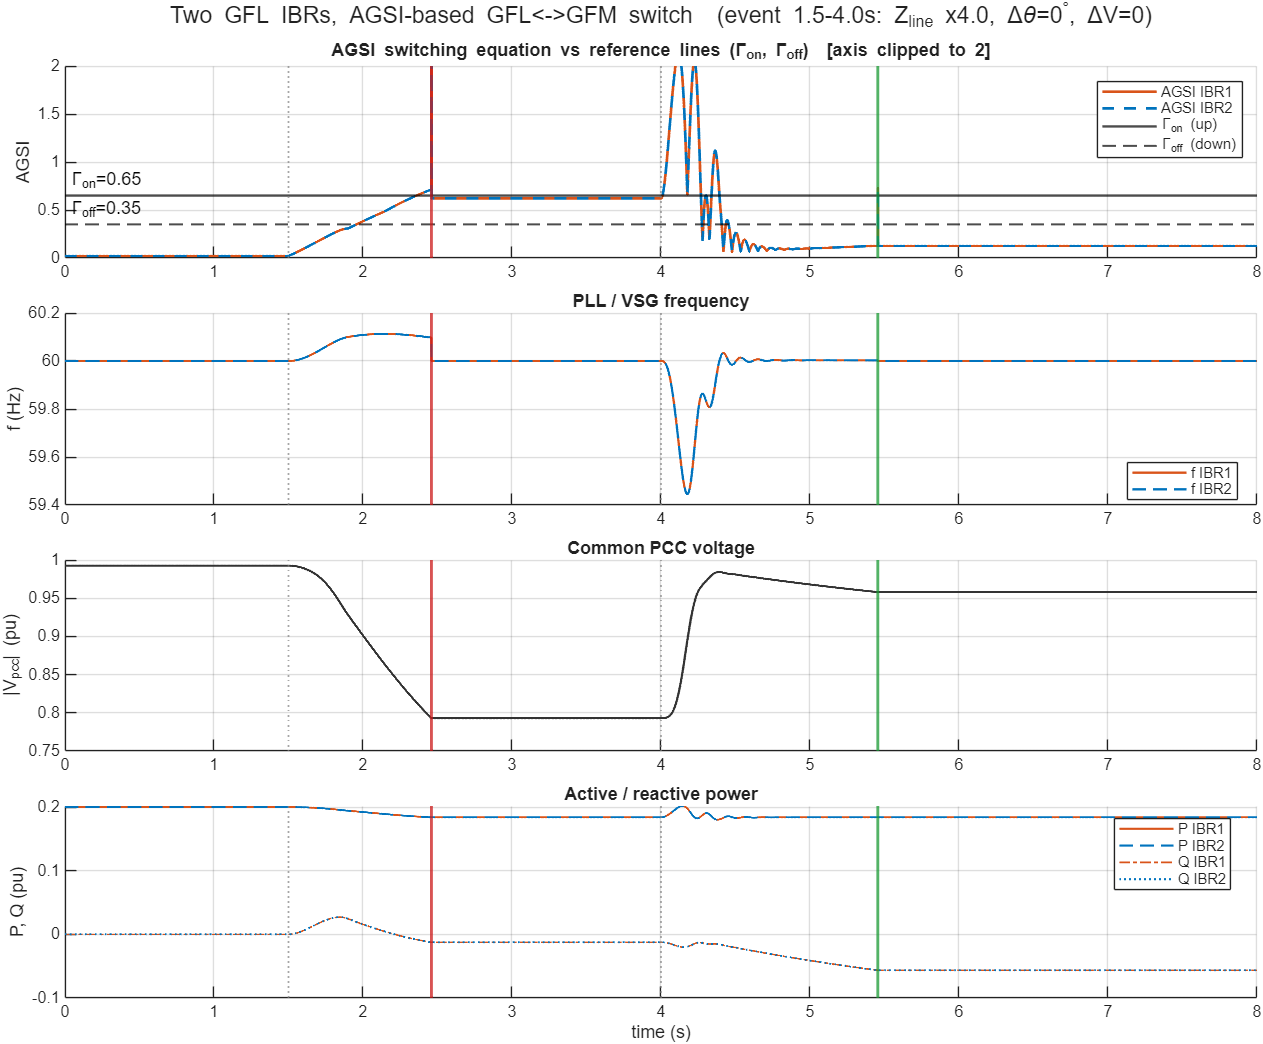
\includegraphics[width=\textwidth]{figures/two_ibr_switch/switch_overview.png}
\caption{ผลรวมสี่แผง: (บน) AGSI เทียบเส้นอ้างอิง (เส้นแดง = GFL$\to$GFM, เส้นเขียว = GFM$\to$GFL)
(ถัดมา) ความถี่ PLL/VSG, แรงดัน PCC, และกำลัง $P,Q$}
\label{fig:overview}
\end{figure}

\noindent \textbf{ลำดับเหตุการณ์:}
\begin{itemize}
\item \textbf{0--1.5 s:} GFL ปกติ AGSI $\approx0.02$ นิ่ง
\item \textbf{1.5 s:} กริดอ่อน ($Z_{line}\times4$) แรงดันตกแบบ S-curve, AGSI ไต่ขึ้น (นำโดย $J_V$)
\item \textbf{$\approx2.46$ s:} AGSI ชน $\Gamma_{on}=0.65$ $\Rightarrow$ สลับเป็น \textbf{GFM}
\item \textbf{2.46--4.0 s:} GFM ประคองกริดอ่อน AGSI ค้างในแถบฮิสเทอรีซิส ความถี่กลับ $60$ Hz
\item \textbf{4.0 s:} กริดคืน แรงดันฟื้น transient สั้น ๆ (dwell กรอง)
\item \textbf{$\approx5.45$ s:} AGSI ตกใต้ $\Gamma_{off}=0.35$ $\Rightarrow$ สลับกลับ \textbf{GFL}
\item \textbf{$>5.45$ s:} GFL ปกติ AGSI $\approx0.13$
\end{itemize}

\noindent \textbf{ยืนยันแล้ว:} วงจรสลับสองทางครบ (\texttt{n\_switch}$=2$/ตัว จบที่ GFL); Newton ลู่เข้าทุกสเต็ป;
กระแสต่อเนื่อง $\sim2.8\times10^{-17}$ ทั้งสองทิศ; ความถี่แกว่ง $\pm0.6$ Hz; สมดุลก่อนเหตุการณ์ residual
machine precision; ทดสอบ \texttt{tests/test\_ibr\_switchable6.m} ผ่านทั้งหมด (รวมเส้นทาง \texttt{solve\_case})

\section{วิธีรัน}
\begin{itemize}
\item คำสั่งเดียว (เด้ง dialog ตั้งค่า): \texttt{run\_two\_ibr\_switch}
\item ข้าม dialog: \texttt{run\_two\_ibr\_switch(Zline\_factor=5)}
\item ผ่าน launcher: \texttt{solve\_case('analysis','ibr','case','two\_ibr\_switch')}
\end{itemize}

\section{สรุปและข้อจำกัด}
กลไกสลับ GFL$\leftrightarrow$GFM ด้วยสมการ AGSI ทำงานถูกต้องสองทาง โปร่งใส และต่อเนื่องกระแส ข้อจำกัด
ที่ระบุตรงไปตรงมา: (1)~น้ำหนัก/เกณฑ์เป็น \texttt{PROJECT\_DERIVED\_SOURCE\_GUIDED} \emph{ไม่ได้} ผ่าน
Bayesian Optimization; (2)~ที่ PCC ร่วม IBR สองตัวเห็นแรงดันเท่ากันจึงสลับพร้อมกัน (เฟสถัดไปควรแยกบัส+tie);
(3)~ตัวขับเป็น diagnostic ไม่ใช่ production TS kernel; (4)~ยังไม่รวม current limiter/LVRT จึงเป็นหลักฐาน
เชิงโครงสร้างของกลไก ไม่ใช่การรับรอง fault-ride-through

\clearpage
\section{การศึกษาขยาย: การสลับโหมดอัตโนมัติบนระบบหลายเครื่องสองระบบ}
ส่วนนี้ขยายการสาธิตแบบ PCC ร่วม ไปสู่ระบบหลายเครื่องสองระบบ ซึ่งมีเครื่องกำเนิดไฟฟ้าซิงโครนัส (SG)
หนึ่งเครื่องใช้โครงข่ายร่วมกับ IBR แบบ grid-following (GFL) หลายตัว เมื่อ SG ถูกปลด (trip) IBR ที่เครียด
จะฟอร์มตัวเป็น GFM (GFL$\to$GFM) เพื่อประคองเกาะ (island) และเมื่อ SG กลับเข้าระบบแบบซิงโครไนซ์
(reclose) SG จะรับหน้าที่ slack (มุมอ้างอิง) คืน แล้ว IBR ส่งการอ้างอิงกลับและกลับสู่โหมด GFL ตามแผนจ่าย
การตัดสินใจใช้ supervisor เดียวกับ AGSI ที่ยกระดับเป็น \textbf{AGSI++} ในรายงานนี้

\subsection{สมการดัชนีการสลับ AGSI / AGSI++ (ฉบับปรับปรุง)}
ดัชนี Adaptive Grid-Support Index คือผลรวมถ่วงน้ำหนักของดัชนีย่อยที่ normalise แล้ว ประเมิน \emph{ต่อ IBR
ทุกสเต็ปเวลา} ดัชนีย่อยหกตัวคือ
\begin{align}
J_V &= \frac{|V-V_{ref}|}{\Delta V_{base}}, &
J_f &= \frac{|f-f_0|}{\Delta f_{base}},\\
J_R &= \frac{|\mathrm{d}f/\mathrm{d}t|}{\Delta R_{base}}, &
J_P &= \frac{|P_{ref}-P|}{\Delta P_{base}},\\
J_{SCR} &= \max\!\Big(0,\ \tfrac{SCR_{crit}}{SCR}-1\Big), &
J_{lock} &= \frac{|v_q|}{\Delta v_{q,base}},
\end{align}
โดยค่าฐาน normalisation และค่าอ้างอิงคือ $\Delta V_{base}=0.10$ pu, $V_{ref}=1.0$;
$\Delta f_{base}=0.50$ Hz, $f_0=60$; $\Delta R_{base}=1.0$ Hz/s (RoCoF); $\Delta P_{base}=0.20$ pu;
$SCR_{crit}=3$ และ $\Delta v_{q,base}=0.10$ ความหมายทีละพจน์: $J_V$ คือความเบี่ยงเบนแรงดัน (ตัวขับหลัก
เมื่อกริดอ่อน), $J_f$ คือความเบี่ยงเบนความถี่ (บ่งชี้ความไม่สมดุลกำลัง), $J_R$ คือ RoCoF (บ่งชี้ความเฉื่อยต่ำ),
$J_P$ คือความคลาดกำลังจริง (ตัวแปลงส่งกำลังตามคำสั่งไม่ไหว), $J_{SCR}$ วัด \emph{ต้นเหตุ} ความแข็งแรงของกริด
โดยตรง (เป็นบวกเมื่อ SCR ต่ำกว่าเกณฑ์อ่อน), และ $J_{lock}$ ใช้ $|v_q|$ เป็นตัวชี้การหลุด lock ของ PLL
ดัชนีรวมคือ
\begin{equation}
\mathrm{AGSI}=w_V J_V + w_f J_f + w_R J_R + w_P J_P + w_{SCR}J_{SCR} + w_{lock}J_{lock}.
\label{eq:agsi2}
\end{equation}
\textbf{น้ำหนัก:} AGSI ธรรมดาใช้ $[w_V,w_f,w_R,w_P]=[0.30,0.30,0.25,0.15]$ (และ $w_{SCR}=w_{lock}=0$);
ส่วน AGSI++ ใช้ $[w_V,w_f,w_R,w_P,w_{SCR},w_{lock}]=[0.25,0.25,0.15,0.10,0.15,0.10]$ (ผลรวม $=1$)
\textbf{เกณฑ์การสลับพร้อมฮิสเทอรีซิสและเวลาหน่วง (dwell):}
\begin{align}
\text{GFL}\to\text{GFM}:&\quad \mathrm{AGSI}\ge\Gamma_{on}=0.65\ \text{คงอยู่ต่อเนื่อง}\ \ge T_{d,on},\\
\text{GFM}\to\text{GFL}:&\quad \mathrm{AGSI}<\Gamma_{off}=0.35\ \text{คงอยู่ต่อเนื่อง}\ \ge T_{d,off}.
\end{align}
เนื่องจาก $\Gamma_{on}>\Gamma_{off}$ ช่วง $[\Gamma_{off},\Gamma_{on}]$ จึงเป็นแถบฮิสเทอรีซิสที่ไม่มีการสลับ
กันการสลับไปมาถี่ ๆ

\textbf{ความแตกต่างสำคัญของ AGSI++:} มีสามส่วน (๑)~กรอง RoCoF ด้วยตัวกรองความถี่ต่ำผ่านอันดับหนึ่ง
(low-pass, ค่าคงเวลา $\tau_R=0.05$ s)
\begin{equation}
\mathrm{RoCoF}^{\text{filt}}_{n}=\mathrm{RoCoF}^{\text{filt}}_{n-1}
  +\alpha\big(\mathrm{RoCoF}^{\text{raw}}_{n}-\mathrm{RoCoF}^{\text{filt}}_{n-1}\big),
\quad \alpha=\min\!\Big(1,\tfrac{\Delta t}{\tau_R}\Big),
\label{eq:rocoffilt2}
\end{equation}
เพื่อ \emph{ปฏิเสธ spike RoCoF หนึ่งแซมเปิล} ที่เกิดตอนเปลี่ยนโครงสร้าง (trip/reclose) ซึ่งเป็นต้นเหตุของ
การสั่น (chatter) เมื่อไม่มี dwell; (๒)~เพิ่ม $J_{SCR}$ ที่วัดความอ่อนของกริดโดยตรง; และ (๓)~เพิ่ม $J_{lock}$
($|v_q|$) ที่จับการหลุด lock ของ PLL ทั้งสามส่วนช่วยให้ดัชนี \emph{มีขอบเขตและไม่สั่น} (รายละเอียดผลใน
\S\ref{sec:F})

\subsection{แบบจำลอง IBR ลดรูป 6 states (ลำดับสถานะและสมการ)}
แต่ละบล็อกหน้าที่ให้สองสถานะพลวัต อินพุตคือ $u=[P_{ref};Q_{ref}]$ บน system base

\textbf{GFL (grid-following)} ลำดับสถานะ (6):
$x=[\,i_d,\ i_q,\ \delta_{\mathrm{PLL}},\ \xi_{\mathrm{PLL}},\ \xi_P,\ \xi_Q\,]$ ได้แก่ กระแส dq ของ
ตัวกรอง L (บน inverter base), มุม SRF-PLL (rad), ตัวปริพันธ์ PI ของ PLL, และตัวปริพันธ์ PI วงนอกของ $P$
และ $Q$ สมการทั้งหมดคือ
\begin{align}
\dot{\delta}_{\mathrm{PLL}} &= k_{p,\mathrm{PLL}}v_q + k_{i,\mathrm{PLL}}\xi_{\mathrm{PLL}}, &
\dot{\xi}_{\mathrm{PLL}} &= v_q,\\
\dot{\xi}_P &= e_P = P_{ref}-P, & \dot{\xi}_Q &= e_Q = Q_{ref}-Q,\\
i_{d,ref} &= k_{p,P}e_P + k_{i,P}\xi_P, & i_{q,ref} &= -(k_{p,Q}e_Q + k_{i,Q}\xi_Q),\\
\dot{i}_d &= \frac{\omega L\, i_q - R_t i_d + v_{td} - v_d}{L/\omega_b}, &
\dot{i}_q &= \frac{-\omega L\, i_d - R_t i_q + v_{tq} - v_q}{L/\omega_b}.
\end{align}
PLL ล็อกกับแรงดันโดยขับ $v_q\to0$; วงนอก $P,Q$ สร้างคำสั่งกระแส $i_{d,ref},i_{q,ref}$; และ current plant
เป็นแบบสัดส่วนพร้อมการ decouple ($\omega L$) GFL จึงเป็น \emph{แหล่งกระแส} ที่พึ่งการวัดแรงดันกริดผ่าน PLL

\textbf{GFM (grid-forming, ไม่มี PLL)} ลำดับสถานะ (6):
$x=[\,i_d,\ i_q,\ \omega,\ \delta,\ E,\ \xi_V\,]$ ได้แก่ กระแส, ความเร็วโรเตอร์เสมือน (pu), มุมโรเตอร์ (rad),
ขนาดแรงดันภายใน, และตัวปริพันธ์ PI แรงดันแกน d สมการคือ
\begin{align}
\dot{\omega} &= \frac{P_{ref}-P-D_v(\omega-1)}{M}, & \dot{\delta} &= \omega_b(\omega-1),\\
\dot{E} &= \frac{k_Q(Q_{ref}-Q)-k_E(E-|V|)}{\tau_E}, & \dot{\xi}_V &= E - v_{gd},\\
i_{q,ref} &= -\big(k_{p,V}(E-v_{gd})+k_{i,V}\xi_V\big), & i_{d,ref} &= k_{p,V}(-v_{gq}),
\end{align}
โดยความสัมพันธ์ที่ปลายทางเป็นแบบ \emph{จับคู่ไขว้แกน (cross-paired)} คือ $v_{gd}=E+X i_q$ และ
$v_{gq}=-X i_d$ VSG swing ให้ virtual inertia (สมการแรก) และวงแรงดันฟอร์มขนาดแรงดัน $E$ เอง GFM จึงเป็น
\emph{แหล่งแรงดันหลังอิมพีแดนซ์} ที่ประคองกริดอ่อนได้ \textbf{ข้อควรรู้:} การจับคู่ไขว้แกนนี้จำเป็น เพราะ
ถ้าจับคู่ \emph{แกนเดียวกัน} (same-axis) วงแรงดันจะกลายเป็นป้อนกลับบวกและ \emph{ไม่เสถียร} การจับคู่ไขว้
($E$ คุม $v_{gd}$ ผ่าน $i_q$) จึงเป็นสิ่งที่ทำให้วงแรงดันเสถียร

\subsection{คลาส SwitchableIbr6 และการถ่ายโอนแบบต่อเนื่องกระแส}
อุปกรณ์ \texttt{SwitchableIbr6} หนึ่งตัวห่อหุ้มแบบจำลองลดรูป 6 states ทั้ง GFL และ GFM เป็น \emph{แกนสมการ
เดียว} (single source of truth) สถานะแอ็กทีฟ \emph{มี 6 มิติเสมอ} การสลับโหมดเป็นแบบ \emph{ต่อเนื่องกระแส
(bumpless)}: โหมดปลายทางถูก re-initialise ให้ตรงกับปลายทาง $(V,P,Q)$ ณ ขณะนั้น ทำให้กระแสฉีดต่อเนื่อง
\begin{equation}
I^{+} = \overline{\left(\tfrac{S}{V}\right)} = I^{-},
\end{equation}
คือกระแสหลังสลับ ($I^+$) เท่ากับก่อนสลับ ($I^-$) พอดี (ไม่มีการกระโดดของกระแสในโครงข่าย) supervisor ของ
AGSI (\S ก่อนหน้า) ตัดสินการสลับ \emph{ต่อ IBR} พร้อมฮิสเทอรีซิสและ dwell สำหรับการศึกษา SG trip/reclose:
เมื่อ SG หลุด IBR ที่เครียดจน AGSI ข้าม $\Gamma_{on}$ จะฟอร์มตัว (GFL$\to$GFM); เมื่อ SG กลับเข้าแบบ
ซิงโครไนซ์ SG รับ slack (มุมอ้างอิง) คืน แล้ว IBR ส่งการอ้างอิงกลับและกลับสู่แผนจ่าย GFL (ดัชนีเป็นตัวตัดสิน
ว่า IBR ตัวใดจะกลับ)

\subsection{เครื่องกำเนิดไฟฟ้าซิงโครนัส: Padiyar model-1.1}
ลำดับสถานะ $[\delta,\omega,E_q',E_d']$ สำหรับโหมด \emph{manual} (สนามคงที่ ไม่มี AVR, 4 สถานะ) หรือ
$[\delta,\omega,E_q',E_d',E_{fd}]$ สำหรับโหมด \emph{avr} (5 สถานะ):
\begin{align}
\dot{\delta} &= \omega_B(\omega-1),\\
\dot{\omega} &= \frac{P_{m,\mathrm{eff}}-T_e-D(\omega-1)}{2H},\qquad
                P_{m,\mathrm{eff}}=P_m-\frac{\omega-1}{R},\\
\dot{E}_q' &= \frac{E_{fd}-E_q'-(X_d-X_d')I_d}{T_{d0}'},\\
\dot{E}_d' &= \frac{-E_d'+(X_q-X_q')I_q}{T_{q0}'},\\
\dot{E}_{fd} &= \frac{K_A(V_{ref}-|V|)-E_{fd}}{T_A}\quad(\text{เฉพาะ avr}).
\end{align}
$P_{m,\mathrm{eff}}$ รวมผลของ droop ของ governor ปฐมภูมิ ($R=\infty$ ปิดการทำงาน); ในโหมด manual
$E_{fd}=E_{fd0}$ คงที่ การแก้ stator (พีชคณิต) คือ
\begin{align}
r_d &= V_d-E_d',\qquad r_q = V_q-E_q',\qquad \mathrm{den}=R_a^2+X_d'X_q',\\
I_d &= \frac{-R_a r_d - X_q' r_q}{\mathrm{den}},\qquad
      I_q = \frac{X_d' r_d - R_a r_q}{\mathrm{den}},\\
T_e &= V_d I_d+V_q I_q+R_a(I_d^2+I_q^2).
\end{align}

\subsection{ระบบทดสอบสองระบบ}
\subsubsection{ระบบที่ 1: Padiyar two-area (จุดทำงานไม่เสถียร)}
SG หนึ่งเครื่องที่บัส~11 (AVR, 5 สถานะ) ร่วมกับ GFL IBR สามตัวที่บัส~1, 2 และ 12 การวิเคราะห์สัญญาณเล็ก
(SSSA) ของระบบรวมขณะ SG ออนไลน์: \textbf{23 สถานะ}, มี \textbf{ค่าเจาะจงในระนาบขวาหนึ่งค่า (RHP)},
$\max\re=+0.058\ \mathrm{s^{-1}}$ จึง \emph{ไม่เสถียรเชิงสัญญาณเล็ก}; โหมดแกว่งที่หน่วงน้อยสุดมี
$f=0.677$ Hz, $\zeta=+0.12$ ลำดับการสลับ (ฟอลต์สามเฟสชั่วคราว $Z_f=j0.1$ pu ที่บัส~3 ช่วง
$1.0$--$1.15$ s จากนั้น SG trip ที่ $2$ s และ reclose ที่ $5$ s ในกรอบ $50$ s):
\begin{enumerate}
\item ช่วง $[0,1)$ s: SG เป็น slack; IBR ทั้งสามตัวเป็น GFL
\item ช่วง $1.0$--$1.15$ s: ฟอลต์ชั่วคราว ($Z_f=j0.1$ pu); IBR ขี่ผ่านฟอลต์ในโหมด GFL
\item $t=2$ s: SG หลุด; IBR ทั้งสามข้าม $\Gamma_{on}$ และฟอร์มตัวเป็น GFM (เกิดเกาะ island)
\item $t=5$ s: reclose แบบซิงโครไนซ์; SG รับหน้าที่ slack คืน และ IBR ส่งการอ้างอิงกลับ
\item $t\to50$ s: เนื่องจากจุดทำงาน \emph{ไม่เสถียร} โหมดช้าจึงโตขึ้นและระบบ \emph{ทรุด} สู่สภาพ all-GFM ด้วย
$V_{end}\approx0.30$ pu
\end{enumerate}
สังเกตว่าการดูผลในช่วงสั้น ๆ (เช่น $<10$ s) เพียงอย่างเดียว ``ดูเหมือนดี'' แต่เป็นภาพลวง เพราะโหมดไม่เสถียรที่ช้ามากต้องใช้
เวลานานกว่าจะเผยตัว (ดู \S\ref{sec:F})

\begin{figure}[H]\centering

\includegraphics[width=0.8\linewidth]{figures/switch_padiyar/padiyar_switch_agsi.png}
\caption{Padiyar two-area: ดัชนี AGSI++ ต่อ IBR (ฟอลต์ $Z_f{=}j0.1$ pu แล้ว SG trip $2$ s, reclose $5$ s; กรอบ $50$ s)}
\end{figure}
\begin{figure}[H]\centering

\includegraphics[width=0.8\linewidth]{figures/switch_padiyar/padiyar_switch_voltage.png}
\caption{Padiyar two-area: แรงดันบัสตลอดวงจร trip/reclose}
\end{figure}
\begin{figure}[H]\centering

\includegraphics[width=0.8\linewidth]{figures/switch_padiyar/padiyar_switch_freq.png}
\caption{Padiyar two-area: ความถี่ของ SG และ IBR}
\end{figure}
\begin{figure}[H]\centering

\includegraphics[width=0.8\linewidth]{figures/switch_padiyar/padiyar_switch_p.png}
\caption{Padiyar two-area: กำลังจริงที่ฉีดเข้าระบบ}
\end{figure}

\subsubsection{ระบบที่ 2: IEEE 14-bus (จุดทำงานเสถียร)}
SG หนึ่งเครื่องที่บัส~1 (manual, ไม่มี AVR, 4 สถานะ) ร่วมกับ GFL IBR สี่ตัวที่บัส~2, 3, 6 และ 8 (ลดรูป 6)
SSSA ของระบบรวม: \textbf{28 สถานะ}, \textbf{ไม่มีค่าเจาะจงในระนาบขวา (RHP = 0)},
$\max\re\approx0$ (มีเพียงโหมดมุมอ้างอิงที่ $\approx0$); โหมดหน่วงน้อยสุดมี $f=0.345$ Hz, $\zeta=+0.267$
จึง \emph{เสถียรเชิงสัญญาณเล็ก} ลำดับการสลับ (ฟอลต์สามเฟสชั่วคราว $Z_f=j0.1$ pu ที่บัส~4 ช่วง
$1.0$--$1.15$ s จากนั้น SG trip ที่ $2$ s และ reclose ที่ $5$ s ในกรอบ $50$ s):
\begin{enumerate}
\item ช่วง $[0,1)$ s: SG เป็น slack; IBR ทั้งสี่ตัวเป็น GFL
\item ช่วง $1.0$--$1.15$ s: ฟอลต์ชั่วคราว ($Z_f=j0.1$ pu); IBR ขี่ผ่านฟอลต์ในโหมด GFL
\item $t=2$ s: SG หลุด; IBR ที่เครียดข้าม $\Gamma_{on}$ และฟอร์มตัวเป็น GFM (เกาะอยู่รอด)
\item $t=5$ s: reclose แบบซิงโครไนซ์; มุมอ้างอิงกลับสู่ SG
\item $t\to50$ s: การตอบสนอง \emph{มีขอบเขต} ($V_{end}\approx0.94$ pu, IBR ส่วนใหญ่กลับสู่ GFL, AGSI มีขอบเขต
ราว $3.5$) แล้วนิ่งเข้าสู่สภาวะคงตัว
\end{enumerate}

\begin{figure}[H]\centering
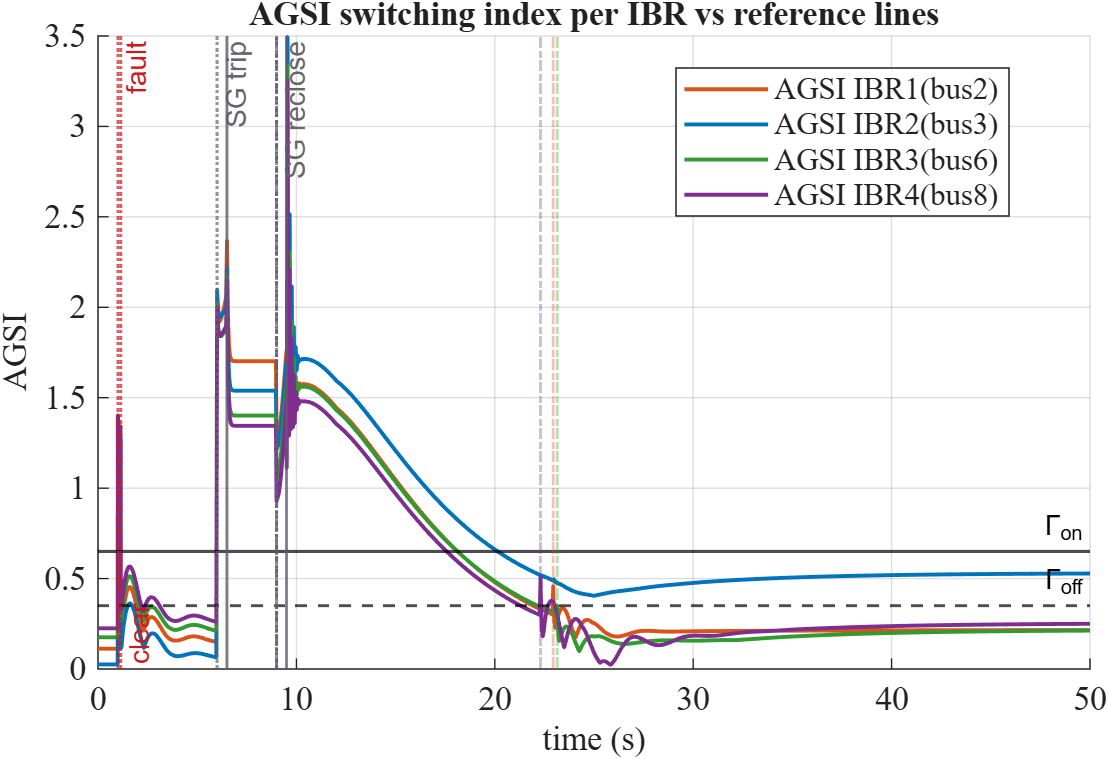
\includegraphics[width=0.8\linewidth]{figures/switch_ieee14/padiyar_switch_agsi.png}
\caption{IEEE 14-bus: ดัชนี AGSI++ ต่อ IBR (ฟอลต์ $Z_f{=}j0.1$ pu แล้ว SG trip $2$ s, reclose $5$ s; กรอบ $50$ s)}
\end{figure}
\begin{figure}[H]\centering
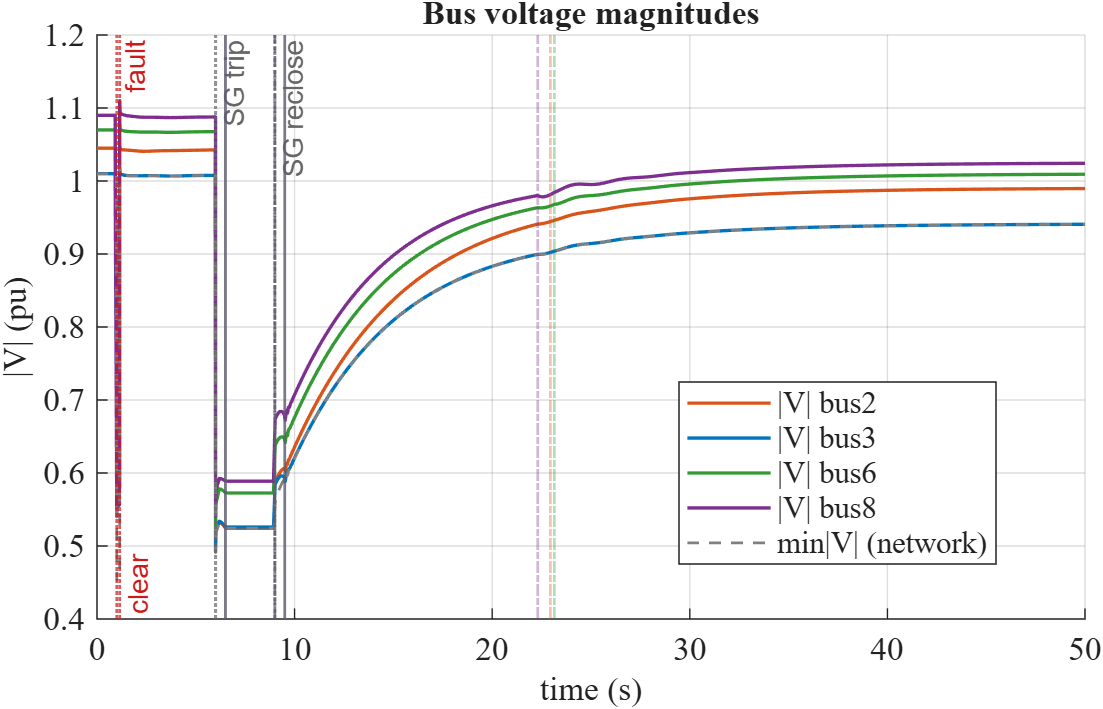
\includegraphics[width=0.8\linewidth]{figures/switch_ieee14/padiyar_switch_voltage.png}
\caption{IEEE 14-bus: แรงดันบัสตลอดวงจร trip/reclose}
\end{figure}
\begin{figure}[H]\centering
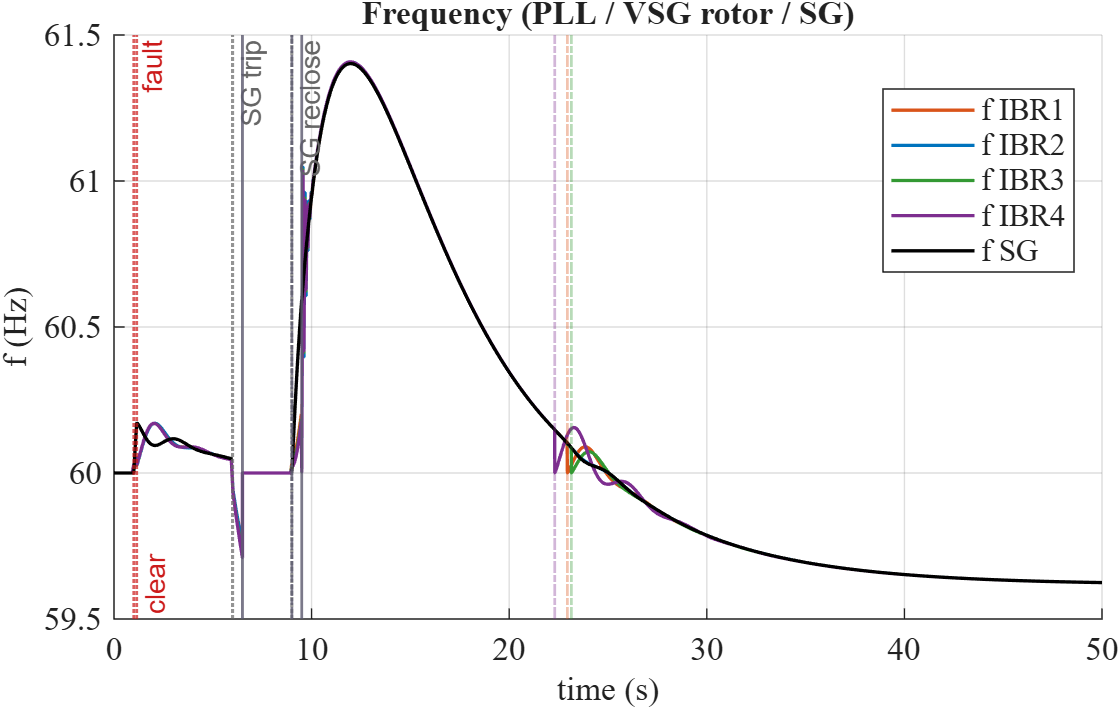
\includegraphics[width=0.8\linewidth]{figures/switch_ieee14/padiyar_switch_freq.png}
\caption{IEEE 14-bus: ความถี่ของ SG และ IBR}
\end{figure}
\begin{figure}[H]\centering
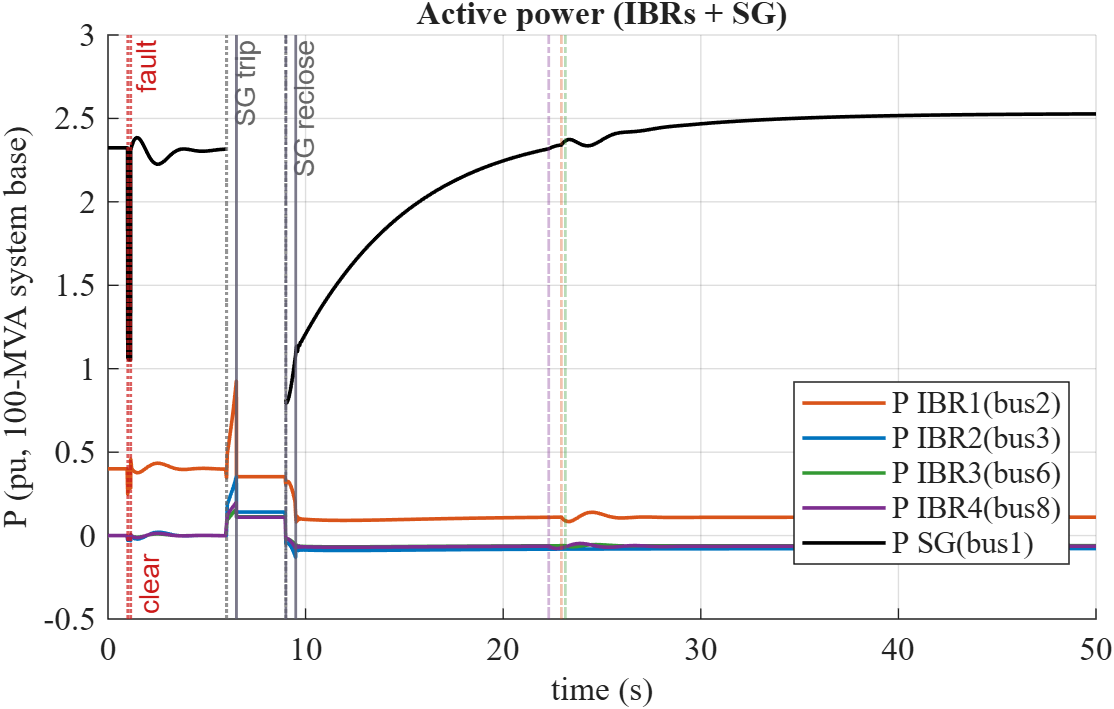
\includegraphics[width=0.8\linewidth]{figures/switch_ieee14/padiyar_switch_p.png}
\caption{IEEE 14-bus: กำลังจริงที่ฉีดเข้าระบบ}
\end{figure}

\section{การวิเคราะห์เชิงลึก}
\label{sec:F}
\subsection{ทำไม Padiyar two-area จึงไม่เสถียร แต่ IEEE 14-bus เสถียร}
ความไม่เสถียรของ Padiyar two-area เป็น \emph{โหมดช้า} (ค่าคงเวลาราว $17$ s, สอดคล้องกับ
$1/0.058\approx17.2$ s) ที่ถูกครอบงำโดย SG เป็นหลัก คือ \emph{มุม/ความเร็วโรเตอร์} ($\delta,\omega$) ร่วมกับ
\emph{ฟลักซ์สนาม} ($E_q'$) แกว่งสวนทางกับกลุ่ม IBR \emph{ผ่านสายเชื่อมสองพื้นที่ (tie-line) ที่อ่อน} และถูก
ซ้ำเติมด้วยสัดส่วน GFL ที่ \emph{สูงมาก} (เกิดปฏิสัมพันธ์ PLL--โครงข่ายในกริดเฉื่อยต่ำและอ่อน) จุดสำคัญคือ
\textbf{ตัว SG เดี่ยว ๆ นั้นเสถียร}: เมื่อวิเคราะห์แบบ SMIB (เครื่องเดียวต่อบัสอนันต์) ได้ $\max\re=-0.248$
(เสถียร) ดังนั้น \emph{การคู่ควบผ่านโครงข่าย (network coupling)} ต่างหากที่ทำให้ไม่เสถียร ไม่ใช่ตัวเครื่องเอง

ในทางกลับกัน IEEE 14-bus เป็นโครงข่าย \emph{ตาข่าย (meshed) พื้นที่เดียว} ที่ \emph{ไม่มีสายเชื่อมระหว่าง
พื้นที่ที่อ่อน} โหมดดังกล่าวจึง \emph{แข็ง (stiff) และหน่วงดี} ระบบจึงเสถียร ข้อสรุปสำคัญ: นี่เป็น
\textbf{ผลของโทโพโลยี (topology effect) ไม่ใช่ผลของ AVR} หลักฐานคือ Padiyar ไม่เสถียรทั้งเมื่อใช้ AVR
($\max\re=+0.058$) และเมื่อใช้ manual ($\max\re=+0.024$) กล่าวคือ ต่อให้ปิด AVR ระบบก็ยังไม่เสถียรจาก
โครงสร้างสายเชื่อมที่อ่อนบวกกับ GFL penetration สูง

\subsection{ประโยชน์ของ AGSI++}
สามส่วนที่เพิ่มใน AGSI++ (RoCoF ที่กรองแล้ว + $J_{SCR}$ + $J_{lock}$) ทำให้ดัชนี \emph{มีขอบเขตและไม่สั่น}
อย่างชัดเจน บนระบบ Padiyar ดัชนี AGSI ฐาน (baseline) พุ่งสูงถึงราว $262$ พร้อมอาการสั่น (chatter) ในขณะที่
AGSI++ มีค่าสูงสุดเพียงราว $2.8$; บน IEEE14 AGSI++ มีค่าสูงสุดราว $3.5$ การกรอง RoCoF กำจัด spike
หนึ่งแซมเปิลที่เกิดตอน trip/reclose (ต้นเหตุหลักของ chatter) ส่วน $J_{SCR}$ และ $J_{lock}$ ทำให้ดัชนีสะท้อน
\emph{ต้นเหตุ} (กริดอ่อน/PLL หลุด lock) แทนที่จะสะท้อนเพียงอาการชั่วขณะ ผลคือการตัดสินสลับสะอาดและเชื่อถือได้
แม้ตั้งค่าให้สลับทันที

\subsection{ผลของเวลาหน่วง (dwell) เปิด/ปิด}
ประเด็นนี้เป็นเหตุผลที่การศึกษานี้ \emph{ต้องใช้ dwell}:
\begin{itemize}
\item \textbf{ไม่มี dwell ($T_d=0$):} หลัง reclose ยอด AGSI ที่ \emph{แตะ} $\Gamma_{on}$ แบบเฉียดฉิว (marginal
peak) เพียงชั่วขณะ ก็เพียงพอจะกระตุ้นการสลับ GFL$\to$GFM \emph{ซ้ำแบบผิดพลาด (spurious re-switch)} เมื่อใด
ที่แหล่งจ่ายทั้งหมดกลายเป็นแบบ grid-forming (GFM หลายตัว + SG) พร้อมกันโดย \emph{ไม่มี headroom ของขีดจำกัด
กระแส} แรงดันจะ \emph{ทรุดแบบหนีตัว (runaway/voltage collapse)}
\item \textbf{มี dwell พอประมาณ ($T_{d,on}=0.5$ s):} เงื่อนไขบังคับให้ AGSI ต้อง \emph{คงอยู่เหนือ}
$\Gamma_{on}$ ต่อเนื่องครบ $0.5$ s ก่อนจึงสลับ ซึ่ง \emph{กรองยอดชั่วขณะ} ทิ้งไป ทำให้ IBR \emph{ยังคงเป็น GFL}
หลัง reclose และทรานเซียนต์หลัง reclose จึง \emph{มีขอบเขต}
\end{itemize}
กล่าวโดยสรุป dwell ทำหน้าที่เป็นตัวกรองเชิงเวลาที่แยก ``ยอดชั่วขณะที่ไม่อันตราย'' ออกจาก ``ภาวะเครียดจริงที่
คงอยู่'' จึงป้องกันการสลับซ้ำผิดพลาดที่นำไปสู่การทรุดของแรงดัน นี่คือเหตุผลเชิงวิศวกรรมที่การศึกษานี้เลือกใช้
เวลาหน่วง

\begin{thebibliography}{9}
\bibitem{eecon49th} EECON49-P4 (KMITL), ``A Bayesian Optimization-Based GFL/GFM Mode Switching
Strategy,'' The 49th Electrical Engineering Conference (EECON-49), 2569.
\bibitem{ding2025b} H. Ding, R. Kar, Z. Miao, and L. Fan, ``A novel design for switchable
grid-following and grid-forming control,'' \emph{IEEE Trans. Sustain. Energy}, vol.~16, no.~2,
pp.~1301--1314, 2025.
\bibitem{liu2024b} P. Liu, X. Xie, and J. Shair, ``Adaptive hybrid grid-forming and grid-following
control of IBRs with enhanced small-signal stability under varying SCRs,'' \emph{IEEE Trans. Power
Electron.}, vol.~39, no.~6, pp.~6603--6607, 2024.
\bibitem{gao2025b} X. Gao, D. Zhou, A. Anvari-Moghaddam, and F. Blaabjerg, ``Seamless switching method
between grid-following and grid-forming control for renewable energy conversion systems,'' \emph{IEEE
Trans. Ind. Appl.}, vol.~61, no.~1, pp.~597--606, 2025.
\bibitem{yazdani2010b} A. Yazdani and R. Iravani, \emph{Voltage-Sourced Converters in Power Systems}.
Wiley-IEEE Press, 2010.
\bibitem{teodorescu2011b} R. Teodorescu, M. Liserre, and P. Rodr\'iguez, \emph{Grid Converters for
Photovoltaic and Wind Power Systems}. Wiley-IEEE Press, 2011.
\bibitem{entsoe_rocof} ENTSO-E, ``Rate of Change of Frequency (RoCoF) withstand capability,''
Network Code RfG implementation guidance document, 2018.
\end{thebibliography}

\end{document}
